\documentclass{standalone}
\usepackage{tikz}
\usetikzlibrary{patterns, positioning}


\begin{document}
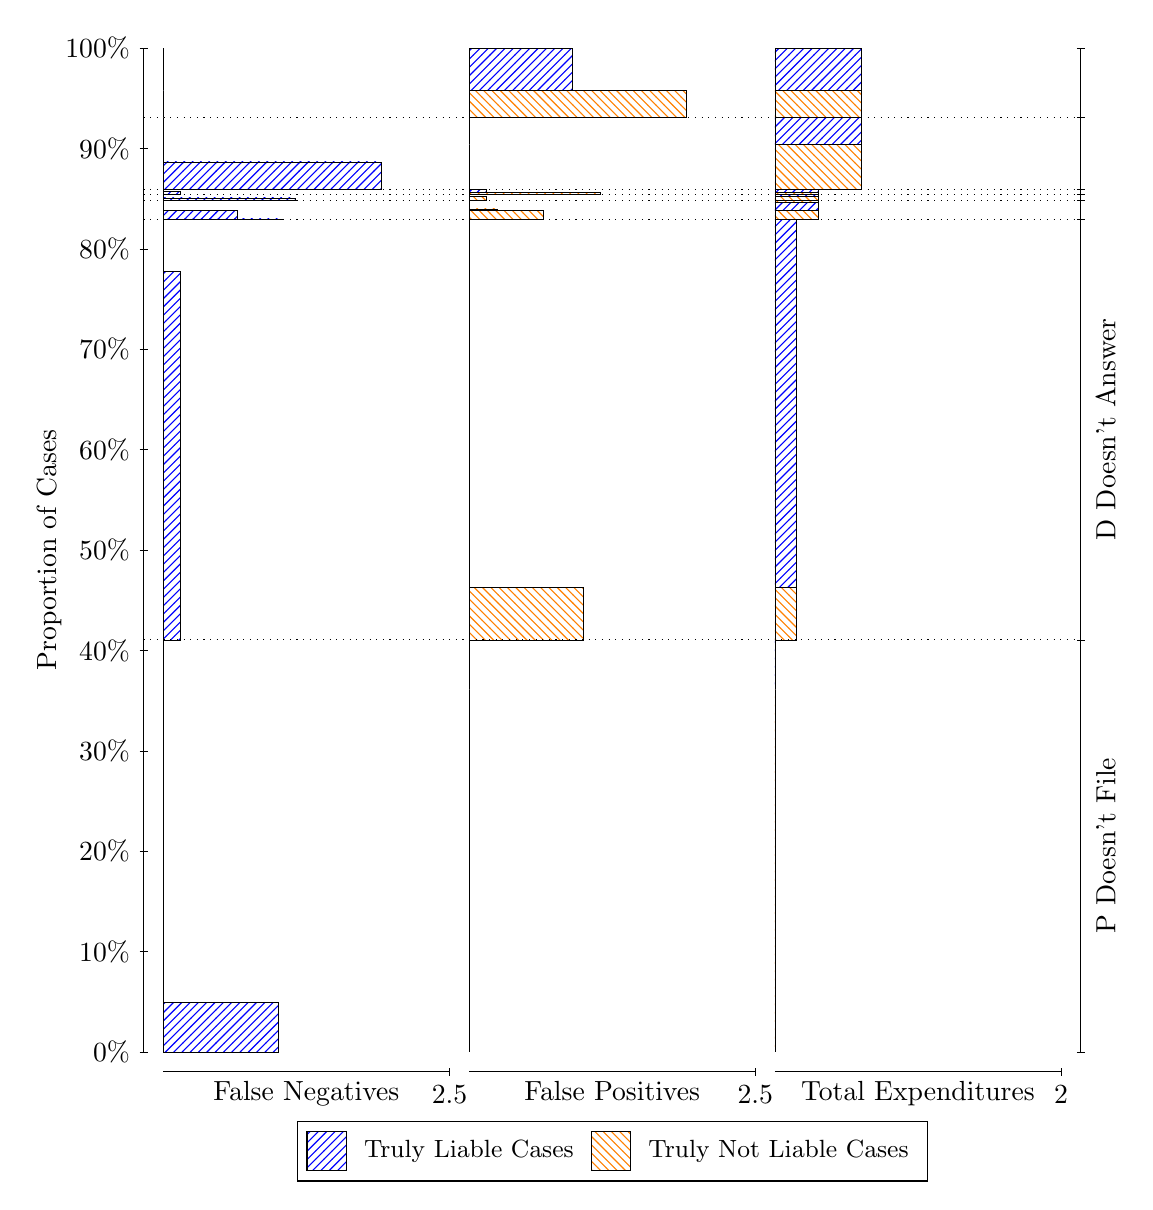
\begin{tikzpicture}
\draw[black, very thin] (1.5,1.75) -- (1.5,14.5);
\node[rotate=90, text=black, anchor=center] at (0.3, 8.125) {Proportion of Cases};
\draw[black, very thin] (1.45,1.75) -- (1.55,1.75);
\node[text=black, anchor=east] at (1.45, 1.75) {0\%};
\draw[black, very thin] (1.45,3.025) -- (1.55,3.025);
\node[text=black, anchor=east] at (1.45, 3.025) {10\%};
\draw[black, very thin] (1.45,4.3) -- (1.55,4.3);
\node[text=black, anchor=east] at (1.45, 4.3) {20\%};
\draw[black, very thin] (1.45,5.575) -- (1.55,5.575);
\node[text=black, anchor=east] at (1.45, 5.575) {30\%};
\draw[black, very thin] (1.45,6.85) -- (1.55,6.85);
\node[text=black, anchor=east] at (1.45, 6.85) {40\%};
\draw[black, very thin] (1.45,8.125) -- (1.55,8.125);
\node[text=black, anchor=east] at (1.45, 8.125) {50\%};
\draw[black, very thin] (1.45,9.4) -- (1.55,9.4);
\node[text=black, anchor=east] at (1.45, 9.4) {60\%};
\draw[black, very thin] (1.45,10.675) -- (1.55,10.675);
\node[text=black, anchor=east] at (1.45, 10.675) {70\%};
\draw[black, very thin] (1.45,11.95) -- (1.55,11.95);
\node[text=black, anchor=east] at (1.45, 11.95) {80\%};
\draw[black, very thin] (1.45,13.225) -- (1.55,13.225);
\node[text=black, anchor=east] at (1.45, 13.225) {90\%};
\draw[black, very thin] (1.45,14.5) -- (1.55,14.5);
\node[text=black, anchor=east] at (1.45, 14.5) {100\%};

\draw[black, very thin] (13.4,1.75) -- (13.4,14.5);
\draw[black, very thin] (13.35,1.75) -- (13.45,1.75);
\node[anchor=west] at (13.35, 1.75) {};
\draw[black, very thin] (13.35,6.9844) -- (13.45,6.9844);
\node[anchor=west] at (13.35, 6.9844) {};
\draw[black, very thin] (13.35,12.327) -- (13.45,12.327);
\node[anchor=west] at (13.35, 12.327) {};
\draw[black, very thin] (13.35,12.568) -- (13.45,12.568);
\node[anchor=west] at (13.35, 12.568) {};
\draw[black, very thin] (13.35,12.639) -- (13.45,12.639);
\node[anchor=west] at (13.35, 12.639) {};
\draw[black, very thin] (13.35,12.709) -- (13.45,12.709);
\node[anchor=west] at (13.35, 12.709) {};
\draw[black, very thin] (13.35,13.618) -- (13.45,13.618);
\node[anchor=west] at (13.35, 13.618) {};
\draw[black, very thin] (13.35,14.5) -- (13.45,14.5);
\node[anchor=west] at (13.35, 14.5) {};

\draw[black, very thin, pattern color=blue, pattern=north east lines] (1.75,1.75) rectangle (3.2033,2.378);
\draw[black, very thin, pattern color=orange, pattern=north west lines] (1.75,2.378) rectangle (1.75,6.9844);
\draw[black, very thin, pattern color=blue, pattern=north east lines] (1.75,6.9844) rectangle (1.968,11.662);
\draw[black, very thin, pattern color=orange, pattern=north west lines] (1.75,11.662) rectangle (1.75,12.327);
\draw[black, very thin, pattern color=blue, pattern=north east lines] (1.75,12.327) rectangle (3.276,12.331);
\draw[black, very thin, pattern color=blue, pattern=north east lines] (1.75,12.331) rectangle (2.6947,12.44);
\draw[black, very thin, pattern color=orange, pattern=north west lines] (1.75,12.44) rectangle (1.75,12.568);
\draw[black, very thin, pattern color=blue, pattern=north east lines] (1.75,12.568) rectangle (3.4213,12.596);
\draw[black, very thin, pattern color=orange, pattern=north west lines] (1.75,12.596) rectangle (1.75,12.639);
\draw[black, very thin, pattern color=blue, pattern=north east lines] (1.75,12.639) rectangle (1.968,12.682);
\draw[black, very thin, pattern color=orange, pattern=north west lines] (1.75,12.682) rectangle (1.75,12.709);
\draw[black, very thin, pattern color=blue, pattern=north east lines] (1.75,12.709) rectangle (4.5113,13.053);
\draw[black, very thin, pattern color=orange, pattern=north west lines] (1.75,13.053) rectangle (1.75,13.618);
\draw[black, very thin, pattern color=orange, pattern=north west lines] (1.75,13.618) rectangle (1.75,13.958);
\draw[black, very thin, pattern color=blue, pattern=north east lines] (1.75,13.958) rectangle (1.75,14.5);
\draw[black, very thin, pattern color=orange, pattern=north west lines] (5.6333,1.75) rectangle (5.6333,6.3564);
\draw[black, very thin, pattern color=blue, pattern=north east lines] (5.6333,6.3564) rectangle (5.6333,6.9844);
\draw[black, very thin, pattern color=orange, pattern=north west lines] (5.6333,6.9844) rectangle (7.0867,7.6496);
\draw[black, very thin, pattern color=blue, pattern=north east lines] (5.6333,7.6496) rectangle (5.6333,12.327);
\draw[black, very thin, pattern color=orange, pattern=north west lines] (5.6333,12.327) rectangle (6.578,12.436);
\draw[black, very thin, pattern color=orange, pattern=north west lines] (5.6333,12.436) rectangle (5.9967,12.456);
\draw[black, very thin, pattern color=blue, pattern=north east lines] (5.6333,12.456) rectangle (5.6333,12.568);
\draw[black, very thin, pattern color=orange, pattern=north west lines] (5.6333,12.568) rectangle (5.8513,12.611);
\draw[black, very thin, pattern color=blue, pattern=north east lines] (5.6333,12.611) rectangle (5.6333,12.639);
\draw[black, very thin, pattern color=orange, pattern=north west lines] (5.6333,12.639) rectangle (7.3047,12.666);
\draw[black, very thin, pattern color=blue, pattern=north east lines] (5.6333,12.666) rectangle (5.8513,12.709);
\draw[black, very thin, pattern color=orange, pattern=north west lines] (5.6333,12.709) rectangle (5.6333,13.273);
\draw[black, very thin, pattern color=blue, pattern=north east lines] (5.6333,13.273) rectangle (5.6333,13.618);
\draw[black, very thin, pattern color=orange, pattern=north west lines] (5.6333,13.618) rectangle (8.3947,13.958);
\draw[black, very thin, pattern color=blue, pattern=north east lines] (5.6333,13.958) rectangle (6.9413,14.5);
\draw[black, very thin, pattern color=orange, pattern=north west lines] (9.5167,1.75) rectangle (9.5167,6.3564);
\draw[black, very thin, pattern color=blue, pattern=north east lines] (9.5167,6.3564) rectangle (9.5167,6.9844);
\draw[black, very thin, pattern color=orange, pattern=north west lines] (9.5167,6.9844) rectangle (9.7892,7.6496);
\draw[black, very thin, pattern color=blue, pattern=north east lines] (9.5167,7.6496) rectangle (9.7892,12.327);
\draw[black, very thin, pattern color=orange, pattern=north west lines] (9.5167,12.327) rectangle (10.062,12.436);
\draw[black, very thin, pattern color=blue, pattern=north east lines] (9.5167,12.436) rectangle (10.062,12.544);
\draw[black, very thin, pattern color=orange, pattern=north west lines] (9.5167,12.544) rectangle (10.062,12.564);
\draw[black, very thin, pattern color=blue, pattern=north east lines] (9.5167,12.564) rectangle (10.062,12.568);
\draw[black, very thin, pattern color=orange, pattern=north west lines] (9.5167,12.568) rectangle (10.062,12.611);
\draw[black, very thin, pattern color=blue, pattern=north east lines] (9.5167,12.611) rectangle (10.062,12.639);
\draw[black, very thin, pattern color=orange, pattern=north west lines] (9.5167,12.639) rectangle (10.062,12.666);
\draw[black, very thin, pattern color=blue, pattern=north east lines] (9.5167,12.666) rectangle (10.062,12.709);
\draw[black, very thin, pattern color=orange, pattern=north west lines] (9.5167,12.709) rectangle (10.607,13.273);
\draw[black, very thin, pattern color=blue, pattern=north east lines] (9.5167,13.273) rectangle (10.607,13.618);
\draw[black, very thin, pattern color=orange, pattern=north west lines] (9.5167,13.618) rectangle (10.607,13.958);
\draw[black, very thin, pattern color=blue, pattern=north east lines] (9.5167,13.958) rectangle (10.607,14.5);
\draw[black, dotted] (1.5,6.9844) -- (13.4,6.9844);
\draw[black, dotted] (1.5,12.327) -- (13.4,12.327);
\draw[black, dotted] (1.5,12.568) -- (13.4,12.568);
\draw[black, dotted] (1.5,12.639) -- (13.4,12.639);
\draw[black, dotted] (1.5,12.709) -- (13.4,12.709);
\draw[black, dotted] (1.5,13.618) -- (13.4,13.618);
\draw[black, very thin] (1.75,1.5) -- (5.3833,1.5);
\node[text=black, anchor=north] at (3.5667, 1.5) {False Negatives};
\draw[black, very thin] (5.3833,1.45) -- (5.3833,1.55);
\node[text=black, anchor=north] at (5.3833, 1.45) {2.5};

\draw[black, very thin] (5.6333,1.5) -- (9.2667,1.5);
\node[text=black, anchor=north] at (7.45, 1.5) {False Positives};
\draw[black, very thin] (9.2667,1.45) -- (9.2667,1.55);
\node[text=black, anchor=north] at (9.2667, 1.45) {2.5};

\draw[black, very thin] (9.5167,1.5) -- (13.15,1.5);
\node[text=black, anchor=north] at (11.333, 1.5) {Total Expenditures};
\draw[black, very thin] (13.15,1.45) -- (13.15,1.55);
\node[text=black, anchor=north] at (13.15, 1.45) {2};

\node[text=black, centered, rotate=90] at (13.72, 4.3672) {P Doesn't File};
\node[text=black, centered, rotate=90] at (13.72, 9.6558) {D Doesn't Answer};






\draw (7.449999999999999,1.5) node[draw=none] (baseCoordinate) {};
\begin{scope}[align=center]
        \matrix[scale=0.5, draw=black, below=0.5cm of baseCoordinate, nodes={draw}, column sep=0.1cm]{
            \node[rectangle, draw, minimum width=0.5cm, minimum height=0.5cm, pattern color=blue, pattern=north east lines] {}; &
            \node[draw=none, font=\small, text=black] (B) {Truly Liable Cases}; &
            \node[rectangle, draw, minimum width=0.5cm, minimum height=0.5cm, pattern color=orange, pattern=north west lines] {}; &
            \node[draw=none, font=\small, text=black] (B) {Truly Not Liable Cases}; \\
            };
\end{scope}

\end{tikzpicture}
\end{document}